\IfFileExists{tables/ablations.tex}{%
  To measure what each design choice contributes, we compare variants of the main setup under an identical budget (same data split, optimiser and number of epochs). Table~\ref{tab:ablations} and Figure~\ref{fig:ablation_curves} report the validation mean AUC; the test set is not used for these comparisons.

  \begin{table}[htbp]
  \centering
  \begin{tabular}{llllrr}
\toprule
Run & Backbone & Loss & Augmentation & Best epoch & Val.\ mean AUC \\
\midrule
base\_5ep & fine-tuned & weighted\_bce & flip & 4/5 & 0.8231 \\
baseline\_frozen & frozen & weighted\_bce & flip & 5/5 & 0.7338 \\
unweighted\_bce & fine-tuned & bce & flip & 4/5 & 0.8360 \\
\bottomrule
\end{tabular}

  \caption{Ablation runs. ``Best epoch'' is the epoch with the highest validation mean AUC.}
  \label{tab:ablations}
  \end{table}

  \begin{figure}[htbp]
  \centering
  \IfFileExists{figures/ablation_curves.png}{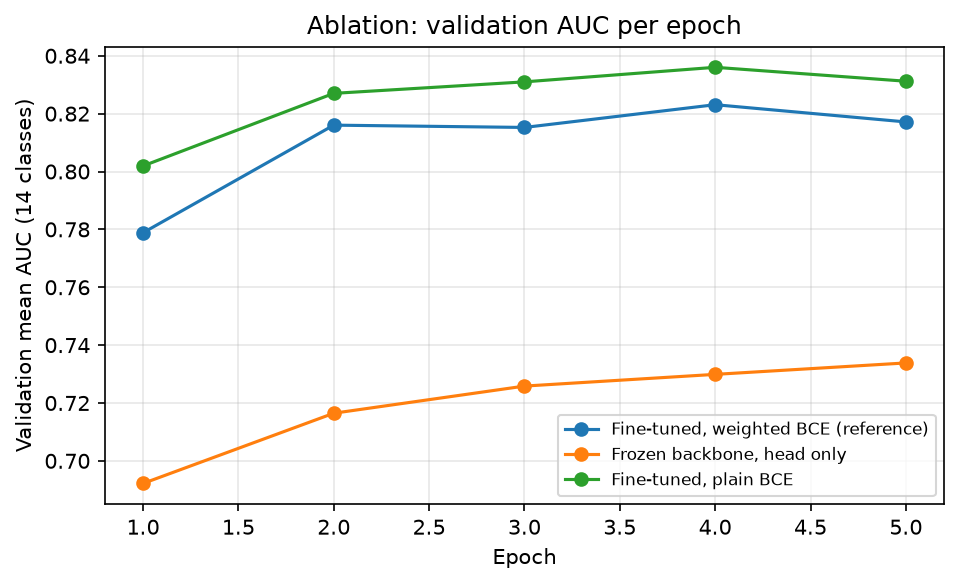
\includegraphics[width=0.75\textwidth]{ablation_curves.png}}{}
  \caption{Validation mean AUC per epoch for each ablation run.}
  \label{fig:ablation_curves}
  \end{figure}

  \paragraph{Fine-tuning matters.} Freezing the backbone and training only the final layer reaches a best validation mean AUC of 0.734, against 0.823 when the whole network is fine-tuned under the same 5-epoch budget. The frozen model is still improving at epoch 5 and both its training and validation losses fall together, so it is limited by capacity to adapt to X-rays rather than by overfitting: ImageNet features alone are not enough for this task.

\paragraph{Weighting the loss did not improve AUC.} Contrary to what we expected, plain binary cross-entropy reached 0.836 against 0.823 for the weighted loss. The plain loss is ahead at every epoch from the second on (by 0.011 to 0.016), and in 13 of the 14 classes at the best epoch, including the rare ones (Hernia $+0.009$, Pneumonia $+0.013$). So in our setup the class weights did not help the ranking quality that AUC measures. We ran a single seed per setting, so a difference of about 0.013 is suggestive and not conclusive, but its consistency across epochs and classes makes a pure fluke unlikely. The weights do change the output scale: the final model's scores are strongly over-confident (mean predicted score 0.38 against a label prevalence of 0.076, Section~\ref{sec:calibration}), which is a plausible side effect of up-weighting positives by factors up to 653. A plain-loss model with a decision threshold chosen on validation is therefore a simpler and, here, better choice. The main model (15 epochs, weighted loss, validation 0.831) was not retrained with plain BCE, and we did not evaluate the plain-loss run on the test set, so we cannot say how much test AUC this would gain.

\paragraph{Overfitting.} In the reference run the validation loss is lowest at epoch 2 (0.977) and then rises to 1.059 at epoch 5 while the training loss keeps falling (1.017 to 0.877); validation AUC peaks at epoch 4 and drops at epoch 5. This is overfitting beginning after three to four epochs. Selecting the best checkpoint by validation AUC, as we do, limits its effect, but it shows that longer training of the main model is not guaranteed to help.

\paragraph{Not run.} A strong-augmentation variant was configured but dropped to save GPU quota, so we make no claim about augmentation. All runs use the same patient-wise split; differences are measured on validation and not on the test set.

}{%
  The planned ablation study (frozen backbone versus fine-tuning, weighted versus plain binary cross-entropy, and the effect of data augmentation) was configured and is reproducible from the repository, but its results were not available when this report was written, so we draw no conclusions about these design choices here.
}
